\documentclass[12pt]{article}
\author{David Alves}

\usepackage{amsfonts}
\usepackage{amsmath}
\usepackage{amsthm}
\usepackage{dirtytalk}
\usepackage[a4paper, total={6.5in, 8.5in}]{geometry}
\usepackage{forest}
\usepackage{skak}
\usepackage{tikz}
\usepackage{titling}
\usepackage{wrapfig}

\def\multichoose#1#2{\ensuremath{\left(\kern-.3em\left(\genfrac{}{}{0pt}{}{#1}{#2}\right)\kern-.3em\right)}}

\title{Math 142 Problem Set 5}
\author{David Alves}
\date{2016-09-27}

\begin{document}
\pagenumbering{gobble}

\begin{center}
\Large \thetitle \\
\large \theauthor \\
\thedate
\end{center}

\subsection*{Sources}

    \begin{itemize}
    \item http://tex.stackexchange.com and https://www.sharelatex.com for help with \LaTeX
    \end{itemize}

\section{Edges in a Complete Graph }

\subsection*{Problem Statement}
Consider a complete graph on 6 vertices. This means that every pair of vertices has exactly one edge between them. How many edges are there in the graph? What if the graph has $n$ vertices?
\subsection*{Solution}

Consider a complete undirected graph $G$ with $n$ vertices. Each edge connects two distinct vertices from the vertex set, and since it is an undirected graph the order of those vertices does not matter. Therefore there is a bijection between the set of edges in $G$ and the set of subsets of length two on a in the vertex set. Therefore there are $\binom{n}{2}$ edges on a complete graph with $n$ vertices. For $n=6$, there are 15 such edges.

\section{Triangles in a Grid}
\subsection*{Problem Statement}
How many triangles can be made with vertices from a $4\times4$ square grid of points? A $2\times2$ square grid would allow 4 triangles. Triangles must use three distinct points and the points cannot be colinear.
\subsection*{Solution}
516 valid triangles can be formed from a grid of $4 \times 4$ points. 
\begin{proof}
    

In a $4 \times 4$ grid there are 16 points. A valid triangle is formed by three distinct noncolinear points. There are $\binom{16}{3} = 560$ ways to choose the three distinct points for a triangle. We know that 560 is equal to the set of valid triangles plus the set of triangles which contain three colinear points by the sum principle. Therefore we can subtract the number of colinear triangles from 560 to determine the number of valid triangles.

    The number of colinear triangles is equal to the number of colinear triangles on rows plus the number of colinear triangles on columns plus the number of colinear triangles on NW-SE diagonals plus the number of colinear triangles on NE-SW diagonals. 
    Each of the four rows contains $\binom{4}{3} = 4$ ways of choosing three colinear points, giving a total of 16 colinear triangles in the rows. By symmetry, there are also 16 colinear triangles in columns. The NE-SW long diagonals also has $\binom{4}{3} = 4$ ways of choosing three colinear points. There are two length-3 NE-SW diagonals, shown here: 

\begin{center}
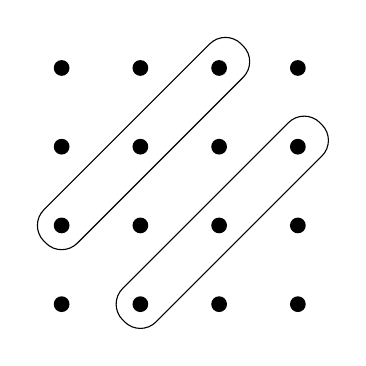
\begin{tikzpicture}
\foreach \x in {0,1,2,3}
    \foreach \y in {0,1,2,3}
    {
    \fill (\x,\y) circle (0.1cm);
    }
\draw[rounded corners=8pt,rotate around={45:(0,1)}] (-.3,.7) rectangle (3.242,1.3);
\draw[rounded corners=8pt,rotate around={45:(1,0)}] (.7,-.3) rectangle (4.242,.3);
\end{tikzpicture}
\end{center}

Each of the length-3 diagonals has $\binom{3}{3} = 1$ way of choosing points for a colinear triangle. This gives $4+1+1 = 6$ colinear triangles on NE-SW diagonals, and therefore 6 on the NW-SE diagonal by symmetry. Thus we have 560 - 16 - 16 - 6 - 6 = 516 noncolinear triangles on a $4 \times 4$ grid of points. 
\end{proof}

\section{Stirling Numbers of the Second Kind}
\subsection*{Problem Statement}
Prove that 
\[
    S(n, m) = \sum_{i=m}^{n}m^{n-i}S(i-1, m-1)
\]
\subsection*{Solution 1}
\begin{proof}
Consider $n$ distinguishable balls being placed into $k$ indistinguishable bins such that each bin contains at least one ball. Without loss of generality, number the balls $b_1, b_2, \ldots, b_n$. Let $b_i$ be the first ball such that $b_1, b_2, \ldots, b_i$ puts at least one ball into each bin. $k \leq i \leq n$ because we need at least $k$ balls to place one in each of $k$ bins. Thus we know that $b_1, b_2, \ldots, b_{i-1}$ require $k-1$ bins. $b_i$ can only be placed into one bin (the empty one). All balls $b_{i+1}, b_{i+2}, \ldots, b_n$ can be placed into any bin since all bins already contain at least one ball. 

The number of ways to place $n$ distinguishable balls into $k$ indistinguishable bins is defined as $S(n,k)$. Thus we can sum over all possible choices of $i$ from $k$ to $n$. For each value of $i$, there are $S(i-1, k-1)$ ways to place the balls before $b_i$ into $k-1$ bins, and $k^{n-i}$ ways to place the balls that come after $b_i$ since they can go into any bin. Thus $S(n,k) = \sum_{i=k}^{n}k^{n-1}S(i-1, k-1)$.
\end{proof}

\subsection*{Solution 2}
\begin{proof}
    The Stirling number of the second kind $S(n,k)$ is defined as the number of ways to divide $n$ items into $k$ groups. Without loss of generality, consider a single item. If that item is in a group by itself, then there are $S(n-1, k-1)$ to partition the remaining items. If that item is not in a group by itself, there are $S(n-1, k)$ ways to partition the remaining items, and the item can go into any of the existing $k$ groups. This leads to the following recurrence relation:

\[
S(n,k) = S(n-1, k-1) + kS(n-1,k)
\]

This recurrence relation can be applied recursively to the $kS(n-1,k)$ term, giving 

\[
S(n,k) = S(n-1, k-1) + k\Big(   S(n-2, k-1) + k\big(   S(n-3, k-1) + k(\ldots )   \big)   \Big)
\]

Multiplying through gives 

\begin{multline*}
    S(n,k) = S(n-1, k-1) + kS(n-2, k-1) + k^2S(n-3, k-1) + \ldots + k^{n-k}S(k-1,k-1) 
\end{multline*}

which can be written as:

\[
\sum_{i=k}^{n}k^{n-1}S(i-1, k-1)
\]
\end{proof}

\section{Squares and Cubes}

\subsection*{Problem Statement}
Show that for all positive integers $n$,
 
\[
    \big(1 + 2 + \ldots + n\big)^2 = 1^3 + 2^3 + \ldots + n^3
\]

\subsection*{Solution}


\begin{proof}
    We prove this by induction on the statement $p(k) = \big(1 + 2 + \ldots + k\big)^2 = 1^3 + 2^3 + \ldots + k^3$. For $k = 1$, $p(1)$ gives $1^2 = 1^3$, which is true. For $k > 1$, we show that if $p(k-1)$ is true, then $p(k)$ is true. First note that the sum of integers $1 + 2 + \ldots + x = \frac{x(x+1)}{2} $. Thus $p(k-1)$ can be written as
    
    \begin{equation}\label{eq:squares1}
    \left(\frac{(k-1)k}{2}\right)^2 = 1^3 + 2^3 + \ldots + (k-1)^3
    \end{equation}
    
    and $p(k)$ can be written as
    \begin{equation}\label{eq:squares2}
    \left(\frac{k(k+1)}{2}\right)^2 = 1^3 + 2^3 + \ldots + k^3 
    \end{equation}
    
    Subtracting equation \ref{eq:squares1} from equation \ref{eq:squares2} gives 
    
    \begin{equation}\label{eq:squares3}
    \frac{k^2(k+1)^2 - k^2(k-1)^2}{4} = k^3
    \end{equation}
    
    Which can be further simplified as follows:
    
    \begin{equation}
    \frac{(k^2+2k+1) - (k^2-2k+1)}{4} = k   
    \end{equation}

    or $\frac{4k}{4} = k$. Thus we have shown that if $p(k-1)$ is true, then $p(k)$ is true, which completes the inductive proof.

\end{proof}

\section{Multisets}
\subsection*{Problem Statement}
Define a \emph{multiset} to be a set that allows multiple copies of any element, knows how many copies of each element are present, but does not know the order. (Example:  $\{2,3,2\} = \{2,2,3\}$, but $\{2,2,3\} \neq \{2,3\}$). What is the number of multisets of size 3 using elements from $[5]$? What about in general (size $m$ using elements from $[n]$?)
\subsection*{Solution}

There are $\binom{7}{5} = 21$ multisets on $[5]$ with 3 elements. More generally, there are $\binom{m+n-1}{n}$ multisets on $[n]$ with $m$ elements. 
\begin{proof}
    There is a bijection between multisets on $[n]$ with $m$ elements and lists of length $m+n-1$ where all elements are either 0 or 1 and exactly $n$ elements are 1. A multiset can be represented as a list of $m$ \say{stars} (0s) and $n-1$ \say{bars} (1s) such that the number of stars before the first bar is the the number of 1s in the multiset, the number of stars before the second bar is the number of 2s in the multiset, etc. For example, the multiset $\{1,3,3\}$ on $[5]$ would be represented as $0,1,1,0,0,1,1$. Thus there are $\binom{m+n-1}{n}$ multisets on $[n]$ with $m$ elements. 
\end{proof}

\section{Time Spent}

I spent about six hours on this problem set. I got stuck for a while on how to intuitively understand the Stirling numbers recurrence. Overall this wasn't a very difficult problem set, but it was useful practice.
\end{document}
